\chapter{Paper I:\@
  Mechanism of \ce{Pd(II)}-mediated\linebreak uncaging reactions % chktex 36
  of propargylic substrates
 }%
\label{ch:paper1}

\begin{citacao}
	\fullcite{Coelho_2019}
\end{citacao}

This work contributes to the development of better~\ce{Pd(II)}-based~\ce{C-O} bond cleavage promoters in the context of bioorthogonal catalysis.
These bioorthogonal approaches,
involving transition metals and biocompatible conditions,
have been recently added to the arsenal of tools for chemical biology and medicinal chemistry for the purpose of activating proteins and prodrugs outside or inside living cells.

Following the literature,
the most common mechanism for this process is the formation of a~\ce{Pd(0)} catalyst,
which then undergoes an oxidative addition with the propargyl group to form an allenylpalladium intermediate.
This intermediate can then be hydrolyzed to produce acetol as a side product and to regenerate the~\ce{Pd(0)}.
A less common mechanism is through a~\ce{Pd(II)}-mediated hydration,
which can form an intermediate that can decompose to form~\ce{Pd(II)} by hydrolysis.

This study consisted of an experimental-computational hybrid investigation on the uncaging of propargyl-protected hydroxyl groups (from the prodrug compound DNPPE in particular) using~\ce{Pd(II)} salts in a phosphate-buffered aqueous medium.
The reactions were monitored by UV-vis spectroscopy and discovered to have a biexponential regime,
consistent with biphasic kinetics.
Two distinct rate constants,
$k_1$ and $k_2$,
were determined --- $k_1$,
with a half-life of 1 hour,
being $15 \times$ faster than $k_2$.
$k_1$ was responsible for two turnovers (at around 20~mol\% of the catalyst),
with $k_2$ showing a sharp increase after two turnovers.

According to what was expected from the literature,
the reaction mechanism was thus hypothesized to consist of either
an intramolecular ligand exchange reduction
or nucleophilic attack by solvent,
either followed by reductive elimination to form~\ce{Pd(0)}
or completing the reaction to form hydrolysed carbopalladate intermediates.
Experiments ruled out that the reaction proceeded through~\ce{Pd(0)}
and showed that the catalyst was likely inhibited by the product.

We thus turned to computational calculations,
making use of data from mass spectroscopies (ESI-HRMS with CID-MS/MS were used) to support the hypothesis
that the reaction proceeds through biphasic kinetics with different rates
and
involves a~\ce{Pd(II)}-mediated anti-Markovnikov hydration of the propargyl group,
followed by~\ce{C-O} bond breaking by~\ce{\beta-O} elimination.
Markovnikov keto intermediates were found to be significantly less favourable than those of the anti-Markovnikov route.
In total, 21 rest states and 23 elementary reactions and equilibria were modelled.

In conclusion,
the study demonstrates that
simple~\ce{Pd(II)} salts acted as a catalyst for~\ce{O}-depropargylation with two phases --- one fast,
but lasting only two turnovers due to product inhibition,
and one slow.
The mechanism for the faster phase involves~\ce{Pd(II)} insertion
with an anti-Markovnikov hydration of the propargyl moiety before the~\ce{C-O} bond is cleaved
through~\ce{\beta-O} elimination.
Although a lot of catalyst is needed for the reaction process to be completed due to product inhibition,
such shortcomings can be rationally overcome in the future
through the design of bulky ligand systems
to prevent strong binding of the product.

\section{Paper}

This work was a joint collaboration between researchers
at the Department of Chemistry at the Federal University of Santa Catarina (UFSC),
the Brazilian Synchrontron Light Laboratory (LNLS),
and the Thomson Mass Spectroscopy Laboratory at the State Univeristy of Campinas.

The work was jointly funded by the Brazilian Council for Technological Development (CNPq),
grant/award number 140485/2017--1,
the Brazilian Synchrotron Light Laboratory (LNLS),
grant/award number 20160243/20170351.

The paper was dedicated to the memory of Professor Faruk José Nome Aguilera (1947--2018).

The publication can be read in full next.

Reprinted with permission from~\fullcite{Coelho_2019}.
Copyright~\citeyear{Coelho_2019}
American~Chemical~Society.

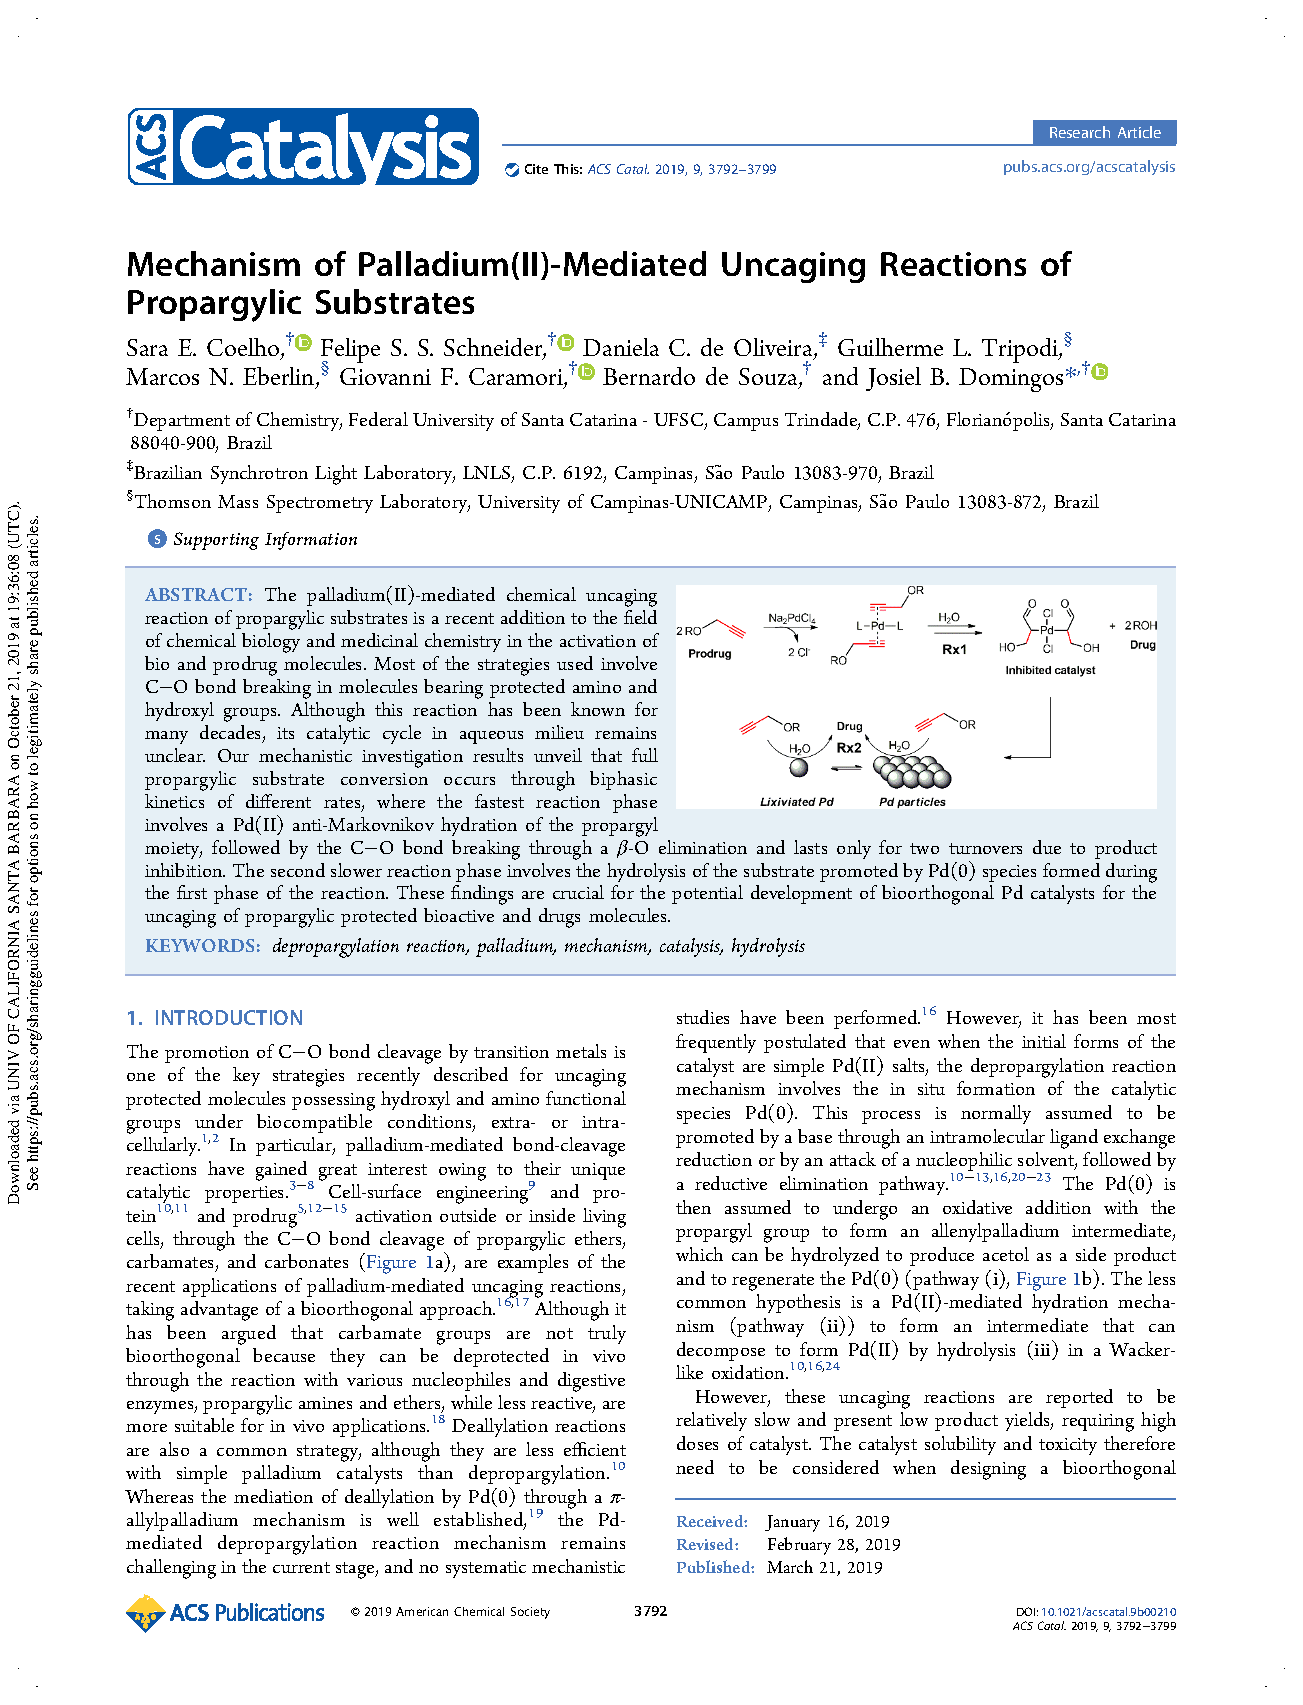
\includepdf[pages=-]{pubs/coelho2019-paper1.pdf}
